%\newcommand{\FigInc}{%
%\begin{wrapfigure}{R}{3.05in}
%  \begin{mdframed}
%  \includegraphics[width=3.0in]{./Figures/Figure.pdf}
%  \caption{An example figure with caption to explain.}
%  \label{incFigure}
%  \end{mdframed}
%\end{wrapfigure}}


\subsubsection{Aim 1: \SpecificAimOne}

\paragraph{Rationale}

Aim 1 focuses on applying the tools used in Gerstung \textit{et al.} alongside the 
GRITIC method to a newly compiled dataset of Black Americans diagnosed with NSCLC. 
This approach is motivated by the need to establish a reliable baseline of 
mutation timing and evolutionary patterns that are specific to this demographic, 
which is often underrepresented in cancer research. 
The Gerstung \textit{et al.} method provides a proven framework 
for analyzing mutational signatures and evolutionary trajectories, 
providing insights into the genetic dynamics of cancer progression. 
The GRITIC method complements this analysis by providing precise timings of sequential copy number gains, 
via a sophisticated MCMC algorithm to unravel complex genetic variations. 
Together, these methods will allow us to map out a mutational landscape, 
providing a foundational analysis, that will be used to compare methodological efficacy 
and validate the model developed in Aim 2. 

\begin{wrapfigure}{R}{2.05in}
  \begin{mdframed}
  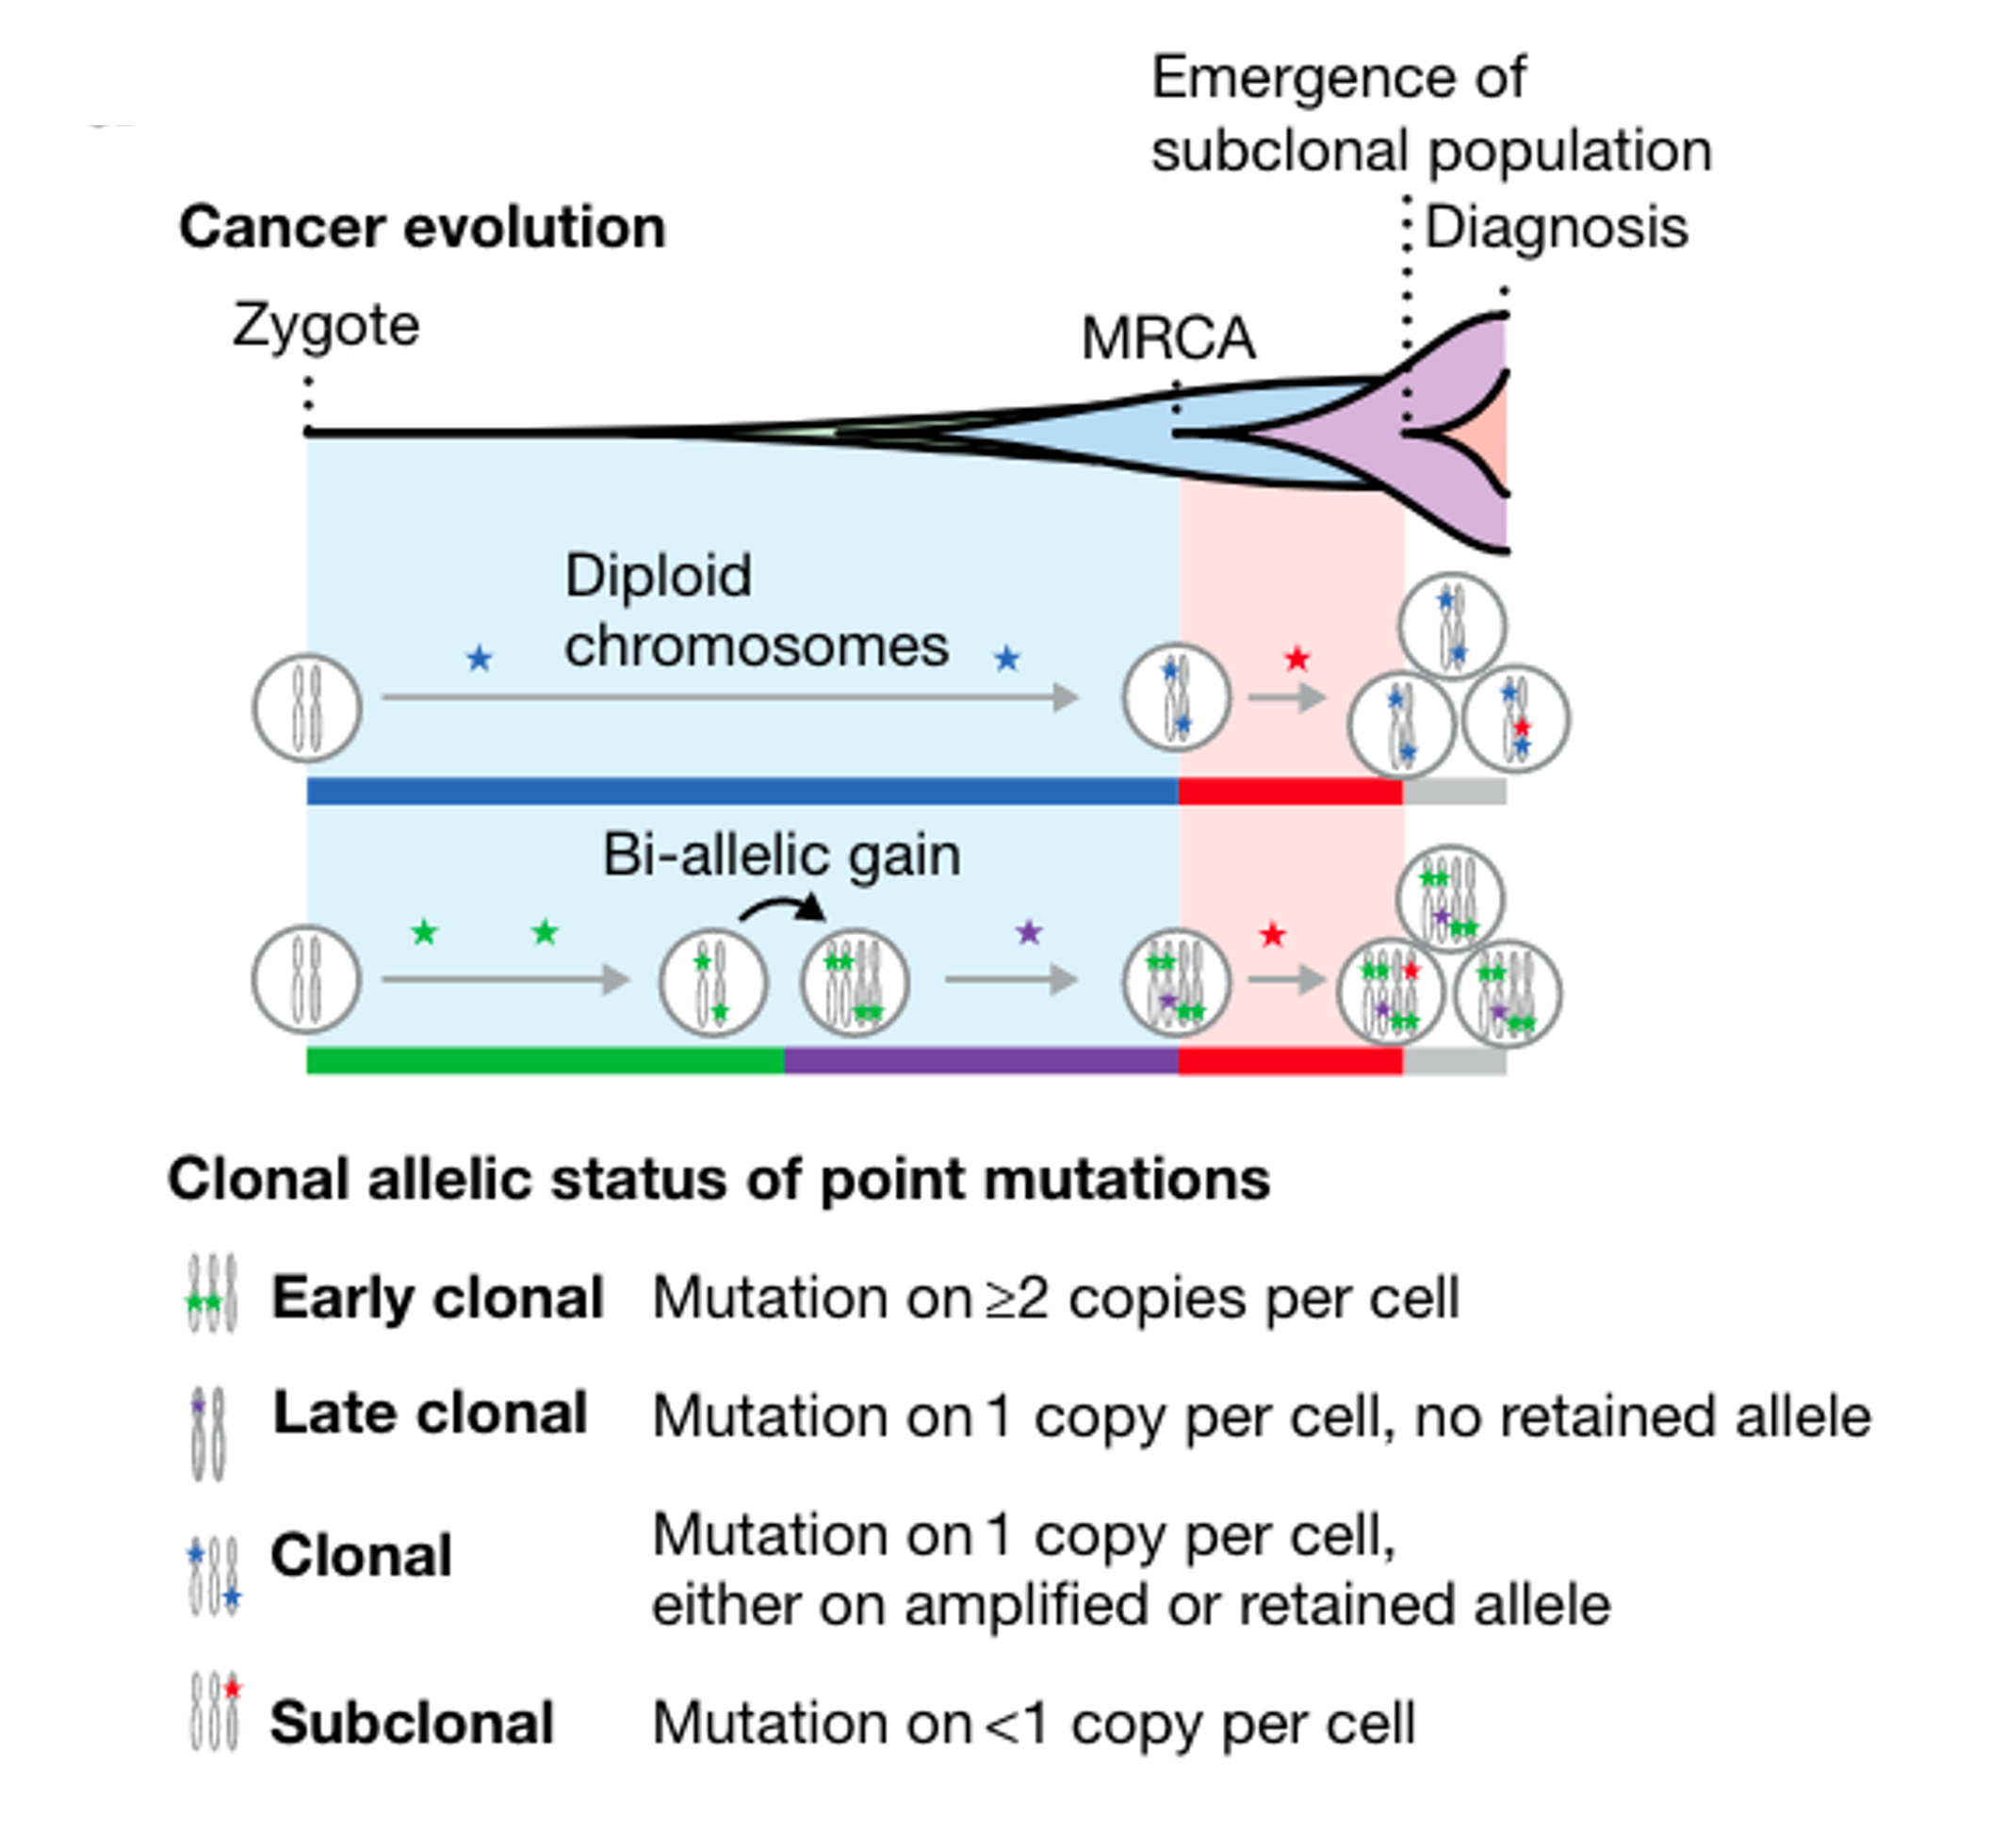
\includegraphics[width=2.0in]{./Figures/definitions.png}
  \caption{Principles of timing mutations and copy number gains based on whole-genome sequencing. 
  Figure from Gerstung \textit{et al.}
  }
  \label{definitions}
  \end{mdframed}
\end{wrapfigure}


\paragraph{1.1. \SpecificAimOneA}

This stage involves collaborating with regional medical centers and 
cancer research networks to collect extensive genomic data from NSCLC patients, 
particularly those of Black American descent. 
The data will undergo rigorous cleaning and processes to remove biases and errors. 
This includes alignment to reference genomes, removing duplicate reads, correcting sequencing errors, 
and accounting for mutations that occur in healthy cells. 
We will also implement stringent quality control measures to validate the integrity and completeness of the data, 
ensuring that it meets the analytical requirements of the computational methods to be applied.
While it may seem trivial, this step is expected to take the longest, 
as it is not always immidiately clear what preprocessing steps are required. 

\paragraph{1.2. \SpecificAimOneB}

In this phase, we will apply the Gerstung \textit{et al.} method to assess mutational signatures and evolutionary trajectories. 
This method will help us statistically model mutation rates and clonal evolution patterns to infer the historical development of tumors. 
We will also use the GRITIC method to analyze sequential copy number gains. 
GRITIC implements an advanced MCMC algorithm to infer the timing and progression of these genetic changes. 
The integration of findings from both methods will allow us to develop a baseline anaysis of tumor evolution in the NCSLC dataset, 
focusing on identifying critical mutational events and their timings.

\begin{figure}[h] % "htbp" here means "here, top, bottom, or on a float page", controlling where the figure is placed
  \centering
  \begin{mdframed}
  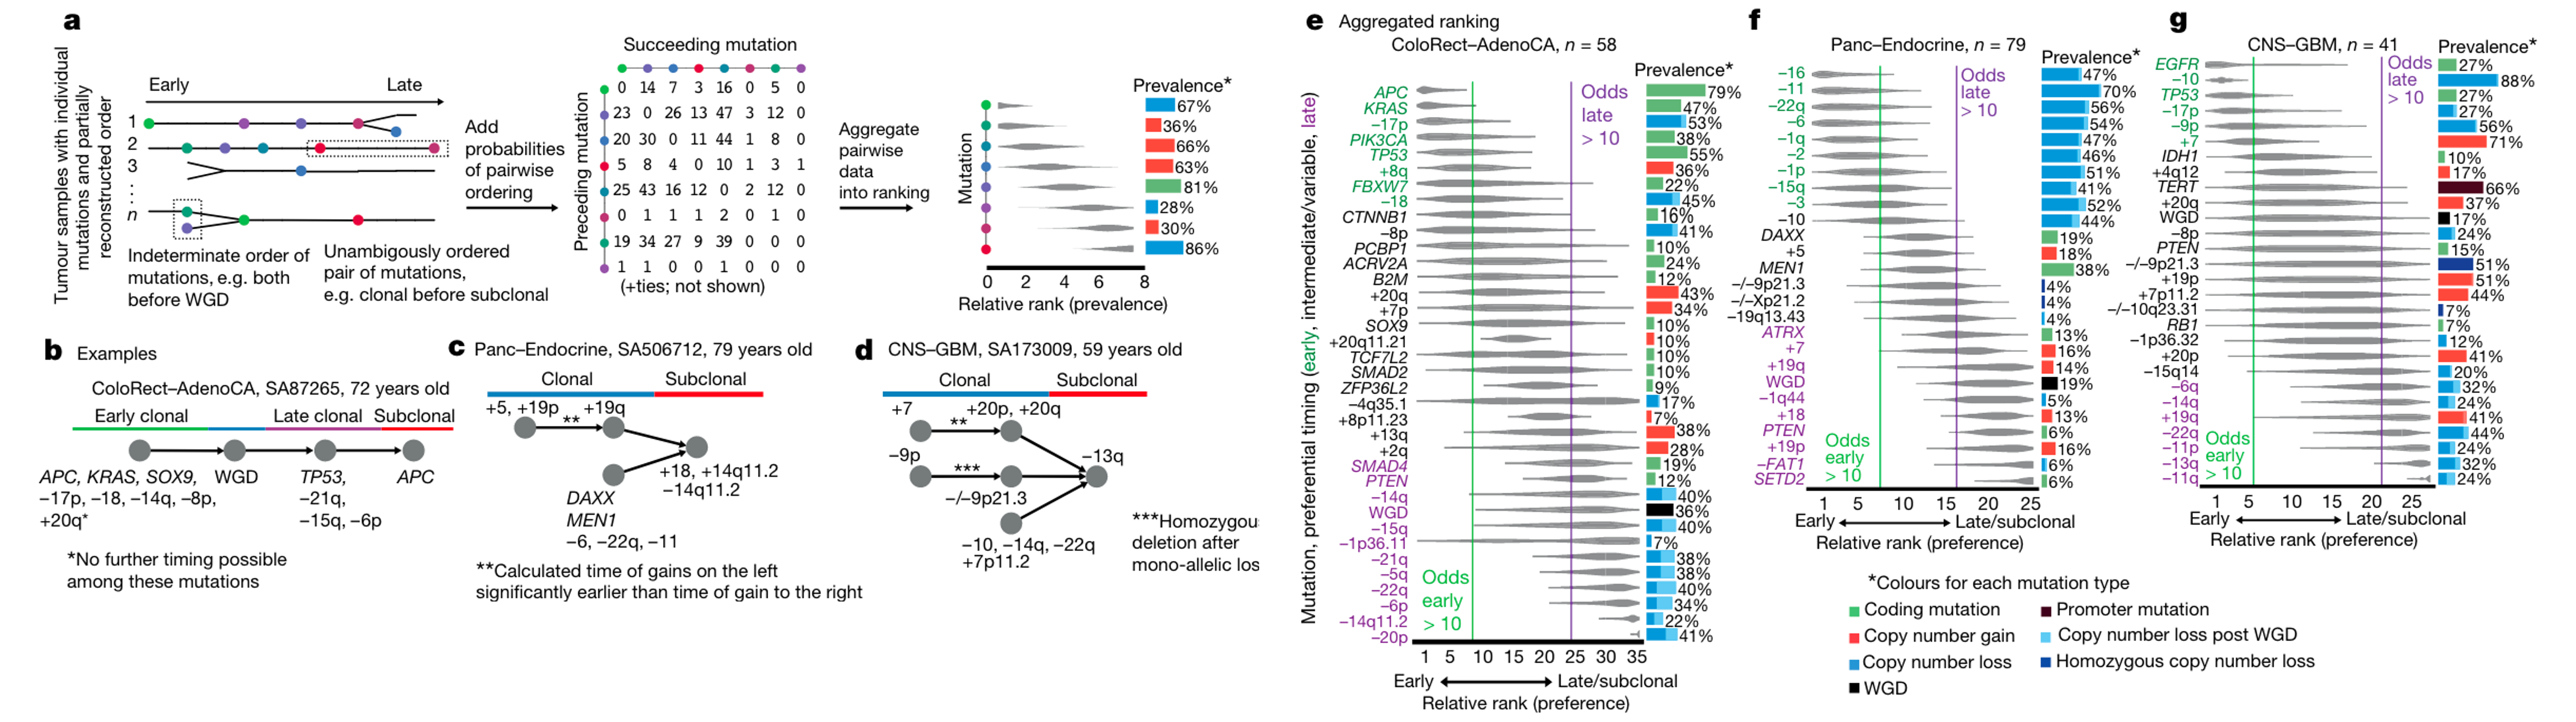
\includegraphics[width=7.4in]{./Figures/driver_mutations_timing.png}
  \caption{Aggregating single-sample ordering reveals typical timing of driver mutations. 
  a, Schematic representation of the ordering process. 
  b–d, Examples of individual patient trajectories (partial ordering relationships), the constituent data for the ordering model process. 
  e–g, Preferential ordering diagrams for colorectal adenocarcinoma (ColoRect–AdenoCA) (e), pancreatic neuroendocrine cancer (Panc–Endocrine) (f) and glioblastoma (CNS–GBM) (g). 
  Probability distributions show the uncertainty of timing for specific events in the cohort.
  Figure from Gerstung \textit{et al.}}
  \label{driver_mutations}
  \end{mdframed}
\end{figure}

\paragraph{1.3. \SpecificAimOneC}

After conducting the computational analyses, we will synthesize the results to highlight key mutational timings and evolutionary patterns. 
A comparative analysis will be performed to align our findings with existing literature on NSCLC, 
especially focusing on unique trends and discrepancies relevant to the Black American population. 
Detailed reports and visual representations, such as evolutionary trees and mutation timelines, 
will be prepared to document these baseline findings comprehensively. 
This documentation will serve as a reference for subsequent analyses.

\begin{wrapfigure}{R}{4.05in}
  \begin{mdframed}
  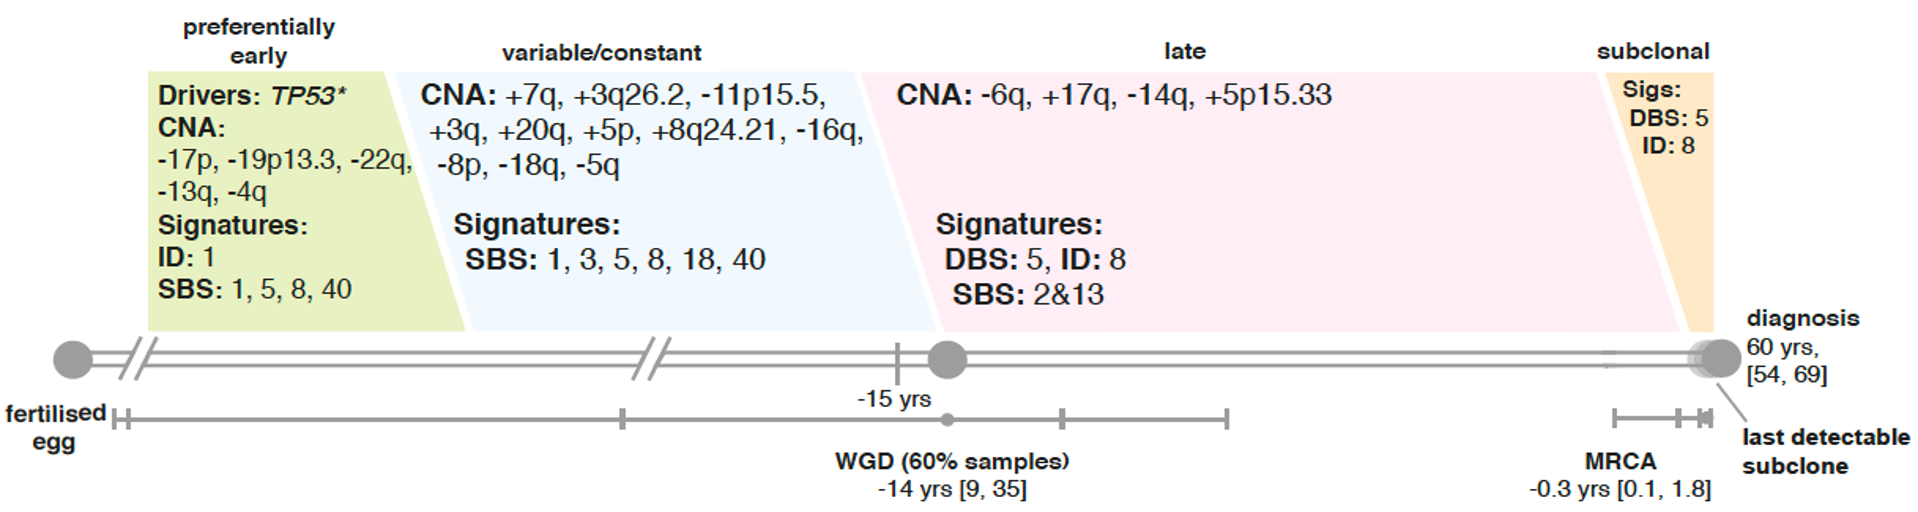
\includegraphics[width=4.0in]{./Figures/evolution-map.png}
  \caption{Timing model for serous ovarian carcinomas. 
  			Estimates on when major events occur during tumor development are provided.~\cite{gerstung_evolutionary_2020}}
  \label{timeline}
  \end{mdframed}
\end{wrapfigure}

\paragraph{Challenges \& Alternative Approaches}

We anticipate challenges such as high inter-individual variability in mutation rates and evolutionary patterns. 
To address this, we plan to incorporate a larger sample size and employ robust statistical methods to ensure the generalizability of our findings. 
The computational demands of the GRITIC method will be managed by leveraging high-performance computing resources 
and optimizing algorithm parameters to enhance computational efficiency without compromising accuracy. 
We will also ensure seamless integration of results from different computational methods by 
using standardized data formats and developing custom scripts for data merging and analysis.
